\chapter{Autodiagnóstico Inicial}

Este capítulo presenta el autodiagnóstico de ContractIA siguiendo la plantilla
estructurada del curso. El objetivo es evaluar honestamente el camino recorrido,
declarar formalmente qué constituye el MVP entregado y documentar los supuestos
y límites que definen su alcance.

\medskip
\noindent\textbf{Distinción clave — prototipo vs. MVP:}
A lo largo del proyecto coexistieron dos estadios del sistema con roles distintos:

\begin{itemize}
    \item \textbf{Prototipo (notebooks v1–v15):} implementación exploratoria en
    Jupyter Notebook, ejecutada localmente, sin API ni despliegue. Su propósito
    fue validar supuestos técnicos: ¿puede un LLM detectar inconsistencias
    contractuales? ¿funciona la segmentación? ¿el RAG recupera contexto útil?
    \item \textbf{MVP (sistema desplegado):} el sistema resultante del
    autodiagnóstico — FastAPI + Cloud Run + bot Telegram + base de datos
    PostgreSQL —, capaz de entregar valor real a un usuario real en un flujo
    de punta a punta, sin intervención del equipo de desarrollo.
\end{itemize}

El autodiagnóstico evalúa el prototipo (punto de partida) para declarar qué
es el MVP (punto de llegada del Capstone II).

% ─────────────────────────────────────────────────────────────────────────────
\section{Información Básica del Equipo}

\begin{table}[H]
\centering
\caption{Información básica del proyecto}
\label{tab:equipo}
\begin{tabular}{p{4cm} p{10cm}}
\toprule
\textbf{Campo} & \textbf{Detalle} \\
\midrule
Nombre del producto & ContractIA \\[4pt]
Equipo & Equipo 4 \\[4pt]
Dominio & Contratos de concesión / Sector público (Estado peruano) \\[4pt]
Descripción del problema &
  Los especialistas de ProInversión invierten $\sim$320 horas en la revisión
  manual de un contrato de concesión APP de 300+ páginas, sin trazabilidad
  sistemática de hallazgos ni cobertura normativa homogénea entre revisores. \\[4pt]
Solución propuesta &
  Agente IA multi-especialista (Jurista + Auditor + Cronista) con RAG híbrido
  (FAISS + BM25 + Cohere Reranker) sobre normativa vectorizada peruana, que
  produce un reporte de inconsistencias trazado en $<1$ hora. \\
\bottomrule
\end{tabular}
\end{table}

% ─────────────────────────────────────────────────────────────────────────────
\section{Estado Actual del Prototipo}

\subsection{¿Qué demostró el prototipo (notebooks v1–v15)?}

El prototipo, desarrollado íntegramente en Jupyter Notebook con ejecución local,
tuvo como único propósito validar la viabilidad técnica de la hipótesis central
\textit{antes} de invertir en infraestructura de producción. Demostró que es
técnicamente posible:

\begin{enumerate}
    \item \textbf{Ingesta y extracción:} Procesar contratos PDF de hasta
    400 páginas con extracción de texto, normalización UTF-8 y detección
    de páginas ilegibles.
    \item \textbf{Segmentación automática:} Detectar capítulos y secciones
    mediante expresiones regulares con mecanismo anti-TOC, logrando
    cobertura del 100\% sobre el Contrato A (324 páginas, 448 cláusulas, 41 secciones).
    \item \textbf{Indexación multinivel:} Construir índices FAISS por
    sección y global para recuperación semántica eficiente.
    \item \textbf{RAG híbrido:} Recuperar contexto normativo relevante
    combinando BM25 (léxico) + FAISS (semántico) con reranking Cohere.
    \item \textbf{Análisis multi-agente:} Ejecutar en paralelo tres agentes
    especializados (Jurista, Auditor, Cronista) que identifican
    inconsistencias jurídicas, estructurales y cronológicas.
    \item \textbf{Generación de reporte:} Producir 119 hallazgos trazados
    (capítulo / sección / cláusula / párrafo) en $\approx$1h 15min.
\end{enumerate}

\noindent Lo que el prototipo \textbf{no hacía}: no tenía API, no estaba
desplegado, no tenía autenticación de usuarios, no persistía resultados en
base de datos y requería ejecución manual celda a celda por el equipo técnico.

\subsection{Del prototipo al MVP}

El autodiagnóstico (este capítulo) fue el instrumento que formalizó la
transición. A partir de los resultados del prototipo se decidió:

\begin{itemize}
    \item Qué funcionalidades pasaban al MVP (flujo de punta a punta validado).
    \item Qué quedaba explícitamente fuera del alcance (ver Sección 4).
    \item Cuáles supuestos del prototipo seguían sin validación con usuarios reales.
\end{itemize}

El \textbf{MVP resultante} es el sistema desplegado en producción: FastAPI en
Google Cloud Run, bot de Telegram con flujo de aprobación, base de datos
PostgreSQL (Cloud SQL) y almacenamiento en Google Cloud Storage. Este sistema
puede ser utilizado por un especialista legal sin intervención del equipo de
desarrollo, cumpliendo el criterio definitorio de un MVP.

\subsection{Supuestos críticos del prototipo aún no validados con usuarios reales}

\begin{table}[H]
\centering
\caption{Supuestos del prototipo pendientes de validación con usuarios reales}
\label{tab:supuestos}
\begin{tabular}{p{5cm} p{5cm} p{4cm}}
\toprule
\textbf{Supuesto} & \textbf{Riesgo si es falso} & \textbf{Cómo validar} \\
\midrule
El especialista confía en los hallazgos IA sin validación manual previa &
El reporte no se usa; el sistema es ignorado &
Sesión de revisión guiada con analistas reales de ProInversión \\
\addlinespace
La estructura jerárquica del contrato es suficientemente uniforme para
la segmentación automática &
Cobertura cae por debajo del 80\% en otros contratos sectoriales &
Prueba con 5 contratos de distintos sectores (energía, agua, vial) \\
\addlinespace
Gemini 2.5 Pro detecta contradicciones procedimentales sutiles con
precisión $\geq85\%$ &
Alta tasa de falsos positivos genera desconfianza en el usuario &
Ground truth manual por dos especialistas independientes \\
\addlinespace
El costo por análisis (\$4–8 en API calls) es aceptable para la
institución &
El modelo no es viable económicamente a escala &
Presupuesto validado con equipo de TI de ProInversión \\
\bottomrule
\end{tabular}
\end{table}

% ─────────────────────────────────────────────────────────────────────────────
\section{Definición del MVP}

\subsection{¿Cuál es la decisión de negocio que habilita el MVP?}

El MVP habilita la siguiente decisión institucional:

\begin{quote}
\textit{``El especialista legal decide si el contrato requiere revisión
especializada inmediata o puede continuar al siguiente paso del flujo,
basándose en el reporte de inconsistencias generado automáticamente
por ContractIA en menos de 1 hora.''}
\end{quote}

Esta es una \textbf{decisión de screening} (primera línea de revisión),
no una decisión final de aprobación. El juicio experto del analista
sigue siendo obligatorio; el agente IA reduce el tiempo de preparación
del análisis.

\subsection{¿Quién es el usuario del MVP?}

\begin{table}[H]
\centering
\caption{Perfil del usuario del MVP}
\label{tab:usuario_mvp}
\begin{tabular}{p{4cm} p{10cm}}
\toprule
\textbf{Atributo} & \textbf{Descripción} \\
\midrule
Rol & Especialista legal / analista de contratos de concesión \\[4pt]
Organización & ProInversión u organismo público similar \\[4pt]
Nivel técnico & Medio (maneja Word, Excel, correo institucional; no es programador) \\[4pt]
Frecuencia de uso & Alta (1–3 contratos por semana en período de revisión) \\[4pt]
Pain point principal &
  Invierte 320 horas en un solo contrato; no tiene trazabilidad de hallazgos. \\[4pt]
Resultado esperado &
  Recibir en $\approx 1$ hora un reporte con todos los hallazgos ubicados y justificados. \\
\bottomrule
\end{tabular}
\end{table}

\subsection{Flujo mínimo de punta a punta}

El flujo mínimo que el MVP debe completar de forma autónoma es:

\begin{enumerate}
    \item El usuario carga el contrato PDF a través del bot de Telegram
    o la API REST.
    \item El sistema extrae el texto, normaliza el contenido y segmenta
    automáticamente las secciones del contrato.
    \item Se construyen los índices FAISS y se vectoriza la base normativa
    de referencia.
    \item El RAG híbrido recupera contexto normativo relevante por sección.
    \item Los tres agentes (Jurista, Auditor, Cronista) analizan cada
    sección en paralelo y generan hallazgos trazados.
    \item El sistema consolida y clasifica los hallazgos por severidad
    (ALTA / MEDIA / BAJA).
    \item El usuario recibe el reporte ejecutivo (PDF/JSON) con la ubicación
    exacta de cada hallazgo y su referencia normativa.
\end{enumerate}

El flujo mínimo que el MVP completa de forma autónoma se ilustra a continuación.
Los pasos 1–6 son ejecutados por el sistema; el paso 7 (naranja) corresponde
a la decisión humana del especialista.

% ── Colores del diagrama ──────────────────────────────────────────────────────
\definecolor{contractiaTeal}{RGB}{38,166,154}
\definecolor{contractiaOrange}{RGB}{242,169,59}
\definecolor{contractiaGray}{RGB}{120,120,120}

\begin{figure}[H]
\centering
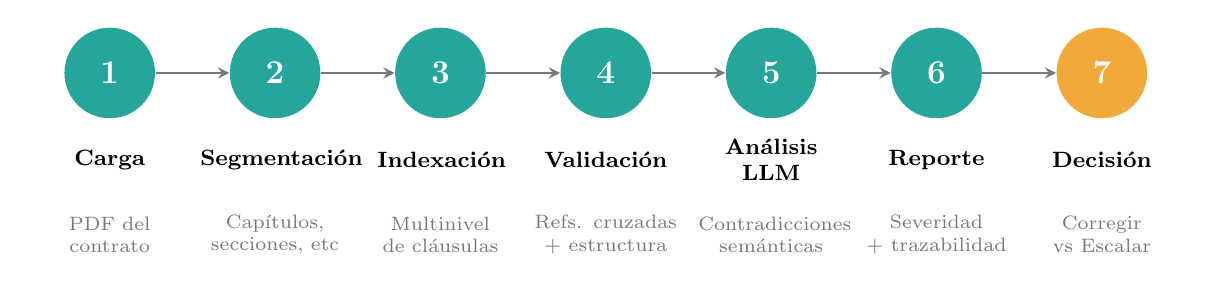
\begin{tikzpicture}[
    % Estilo base para todos los nodos circulares
    stepnode/.style={
        circle, minimum size=1.15cm, inner sep=0pt,
        font=\large\bfseries\color{white}
    },
    % Nodos teal (pasos automáticos)
    tealnode/.style={stepnode, fill=contractiaTeal},
    % Nodo naranja (decisión humana)
    orangenode/.style={stepnode, fill=contractiaOrange},
    % Flecha entre nodos
    myarrow/.style={->, >=stealth, thick, color=contractiaGray},
    % Etiqueta principal (negrita)
    mainlabel/.style={
    font=\footnotesize\bfseries, % Cambiado de \small a \footnotesize
    text centered,
    text width=1.6cm,            % Reducimos un poco el ancho para compensar
    color=black
    },
    % Etiqueta secundaria (descripción)
    sublabel/.style={
        font=\scriptsize, text centered,
        text width=1.85cm, color=contractiaGray
    },
]

%% ── Nodos ────────────────────────────────────────────────────────────────────
\node[tealnode]   (n1) at (0,0)    {1};
\node[tealnode]   (n2) at (2.1,0)  {2};
\node[tealnode]   (n3) at (4.2,0)  {3};
\node[tealnode]   (n4) at (6.3,0)  {4};
\node[tealnode]   (n5) at (8.4,0)  {5};
\node[tealnode]   (n6) at (10.5,0) {6};
\node[orangenode] (n7) at (12.6,0) {7};

%% ── Flechas ──────────────────────────────────────────────────────────────────
\draw[myarrow] (n1) -- (n2);
\draw[myarrow] (n2) -- (n3);
\draw[myarrow] (n3) -- (n4);
\draw[myarrow] (n4) -- (n5);
\draw[myarrow] (n5) -- (n6);
\draw[myarrow] (n6) -- (n7);

%% ── Etiquetas principales ────────────────────────────────────────────────────
\node[mainlabel] at (0,   -1.1) {Carga};
\node[mainlabel] at (1.95, -1.1) {Segmentación};
\node[mainlabel] at (4.2, -1.1) {Indexación};
\node[mainlabel] at (6.3, -1.1) {Validación};
\node[mainlabel] at (8.4, -1.1) {Análisis LLM};
\node[mainlabel] at (10.5,-1.1) {Reporte};
\node[mainlabel] at (12.6,-1.1) {Decisión};

%% ── Etiquetas secundarias ────────────────────────────────────────────────────
\node[sublabel] at (0,   -2.05) {PDF del\\contrato};
\node[sublabel] at (2.1, -2.05) {Capítulos,\\secciones, etc};
\node[sublabel] at (4.2, -2.05) {Multinivel\\de cláusulas};
\node[sublabel] at (6.3, -2.05) {Refs. cruzadas\\+ estructura};
\node[sublabel] at (8.4, -2.05) {Contradicciones\\semánticas};
\node[sublabel] at (10.5,-2.05) {Severidad\\+ trazabilidad};
\node[sublabel] at (12.6,-2.05) {Corregir\\vs Escalar};

\end{tikzpicture}
\caption{Flujo mínimo de punta a punta del MVP ContractIA (pasos 1--6 automáticos; paso 7 humano).}
\label{fig:flujo_e2e}
\end{figure}

% ─────────────────────────────────────────────────────────────────────────────
\section{Definición de Alcance del MVP}

\subsection{¿Qué NO es parte del MVP?}

Las siguientes funcionalidades fueron conscientemente excluidas del MVP
para mantener el foco en la hipótesis central:

\begin{itemize}
    \item \textbf{Interfaz web con diseño final:} La UI de Streamlit/Telegram
    es funcional pero sin diseño gráfico institucional ni sistema de roles.
    \item \textbf{Procesamiento concurrente multiusuario:} El prototipo
    procesa un contrato a la vez (semáforo asyncio); no hay paralelismo
    en GPU ni colas distribuidas.
    \item \textbf{Integración con repositorios documentales:} No hay
    conexión con sistemas SEACE, INFOBRAS u otros repositorios
    institucionales.
    \item \textbf{Modelos predictivos de riesgo:} No se incluye análisis
    longitudinal ni clasificación predictiva de riesgo contractual.
    \item \textbf{Multi-idioma y multi-jurisdicción:} El sistema está
    optimizado exclusivamente para contratos en español bajo normativa peruana.
    \item \textbf{Logging institucional y auditoría de acciones:} No hay
    trazabilidad de acciones de usuario ni políticas de retención documental.
    \item \textbf{Certificación o firma digital:} El reporte es un documento
    de análisis, no un instrumento legal firmado.
\end{itemize}

\subsection{Decisiones ``feo pero funcional'' del MVP}

Estas decisiones fueron tomadas conscientemente para entregar valor
demostrable en el tiempo del proyecto:

\begin{itemize}
    \item El bot de Telegram usa autenticación por lista blanca de
    usernames en lugar de SSO institucional.
    \item Los reportes se generan en JSON/Markdown sin plantilla
    institucional formateada.
    \item La base normativa vectorizada cubre solo las normas principales
    de contratación APP; no incluye normas sectoriales específicas.
    \item La segmentación asume estructura jerárquica decimal estándar;
    contratos con formatos no convencionales pueden requerir ajuste manual.
    \item No hay mecanismo de feedback del usuario para corregir hallazgos
    incorrectos; la retroalimentación es manual.
\end{itemize}

% ─────────────────────────────────────────────────────────────────────────────
\section{Arquitectura Mínima Operable}

\subsection{Componentes del sistema}

\begin{table}[H]
\centering
\caption{Componentes de la arquitectura mínima operable}
\label{tab:arquitectura_mvp}
\begin{tabular}{p{2.8cm} p{4cm} p{6cm}}
\toprule
\textbf{Capa} & \textbf{Componente} & \textbf{Descripción} \\
\midrule
Datos &
  Contratos PDF + Base normativa &
  PDFs de concesión cargados por usuario; normativa peruana APP
  pre-vectorizada (FAISS). \\
\addlinespace
Procesamiento &
  Pipeline de extracción y segmentación &
  PyMuPDF para extracción de texto; regex + anti-TOC para segmentación
  jerárquica; indexación FAISS + BM25. \\
\addlinespace
Modelo &
  Multi-agente LLM + RAG híbrido &
  Gemini 2.5 Pro (Jurista, Auditor, Cronista) vía Vertex AI;
  RAG con FAISS + BM25 + Cohere Reranker. \\
\addlinespace
Salida &
  Reporte ejecutivo + API REST + Bot &
  Reporte JSON/PDF con hallazgos trazados; FastAPI en Cloud Run;
  bot Telegram con flujo de aprobación. \\
\bottomrule
\end{tabular}
\end{table}

\definecolor{archNavy}{RGB}{22,38,74}
\definecolor{archBlue}{RGB}{45,95,175}
\definecolor{archVtx}{RGB}{66,133,244}
\definecolor{archBg}{RGB}{237,239,244}
\definecolor{archBorder}{RGB}{160,175,200}
\definecolor{archArrow}{RGB}{80,95,120}

\begin{landscape}
\begin{figure}[p]
\centering
\begin{tikzpicture}[
    hexL/.style={regular polygon, regular polygon sides=6, minimum size=1.35cm,
        inner sep=2pt, fill=archNavy, draw=archNavy!80!black,
        text=white, font=\footnotesize\bfseries, align=center},
    hexS/.style={regular polygon, regular polygon sides=6, minimum size=0.9cm,
        inner sep=1pt, fill=archBlue, draw=archBlue!80!black,
        text=white, font=\scriptsize\bfseries, align=center},
    vtxdia/.style={diamond, minimum width=1.35cm, minimum height=1.35cm,
        inner sep=0pt, fill=archVtx, draw=archVtx!80!black,
        text=white, font=\scriptsize\bfseries, align=center},
    netcir/.style={circle, minimum size=1.05cm, inner sep=2pt,
        fill=archBlue!80, draw=archBlue, text=white,
        font=\scriptsize\bfseries, align=center},
    smallrec/.style={rounded corners=3pt, minimum width=1.6cm, minimum height=0.7cm,
        inner sep=3pt, fill=archBlue!70, draw=archBlue!90,
        text=white, font=\scriptsize\bfseries, align=center},
    docrec/.style={rectangle, minimum width=0.95cm, minimum height=1.1cm,
        fill=red!60!orange!80, draw=red!70, text=white,
        font=\tiny\bfseries, align=center},
    cicdbox/.style={rounded corners=4pt, draw=archBorder, fill=white,
        align=left, inner sep=7pt},
    contbox/.style={rounded corners=8pt, dashed, thick,
        draw=archBorder, fill=archBg},
    hdr/.style={font=\small\bfseries, color=archNavy, align=center},
    lbl/.style={font=\tiny, color=gray!85!black, align=center, text width=2.1cm},
    arr/.style={dashed, ->, >=Stealth, thick, color=archArrow},
    biarr/.style={dashed, <->, >=Stealth, thick, color=archArrow},
]

%% ─── NODOS ───────────────────────────────────────────────────────────────────
%% Motor Agentes
\node[hexL] (orch)  at (1.5, 3.2)  {};
\node[hexS] (jur)   at (3.6, 4.6)  {J};
\node[hexS] (aud)   at (3.6, 3.2)  {A};
\node[hexS] (cro)   at (3.6, 1.8)  {C};

%% API REST (hub central)
\node[hexL] (api)   at (6.5, 3.2)  {};

%% Motor RAG
\node[vtxdia]  (vtx)   at (9.4,  5.0) {Vertex\\AI};
\node[netcir]  (faiss) at (11.6, 5.0) {FAISS};
\node[smallrec](bm25)  at (9.4,  3.1) {BM25};
\node[smallrec](coh)   at (11.6, 3.1) {Cohere\\Reranker};
\node[netcir]  (grag)  at (10.5, 1.4) {Graph\\RAG};

%% Data Lake
\node[hexL]   (dbapi) at (15.8, 4.2) {};
\node[docrec] (docs)  at (15.8, 1.8) {PDF\\DOCX};

%% CI/CD
\node[cicdbox] (cicd) at (19.5, 6.5) {
    {\small\bfseries CI / CD}\\[3pt]
    {\tiny GitHub Actions $\rightarrow$ Docker}\\
    {\tiny Artifact Registry $\rightarrow$ Cloud Run}
};

%% Interfaces (abajo)
\node[hexL]    (web)  at (2.5,  -1.8) {};
\node[hexS]    (tg)   at (6.5,  -1.8) {};
\node[smallrec](mail) at (10.5, -1.8) {Email};

%% ─── FLECHAS ─────────────────────────────────────────────────────────────────
\draw[arr]   (orch.north east) -- (jur.west);
\draw[biarr] (orch.east)       -- (aud.west);
\draw[arr]   (orch.south east) -- (cro.west);
\draw[biarr] (aud.east)        -- (api.west);
\draw[biarr] (api.east)        -- (vtx.west);
\draw[arr]   (vtx.east)        -- (faiss.west);
\draw[arr]   (bm25.east)       -- (coh.west);
\draw[arr]   (faiss.south) to[bend right=15] (grag.north east);
\draw[arr]   (coh.south)   to[bend left=15]  (grag.north);
\draw[biarr] (faiss.east)      -- (dbapi.west);
\draw[arr]   (dbapi.south)     -- (docs.north);
\draw[arr]   (api.south) to[bend right=20] (web.north);
\draw[arr]   (api.south)       -- (tg.north);
\draw[arr]   (api.south) to[bend left=20]  (mail.north);

%% ─── CONTENEDORES ────────────────────────────────────────────────────────────
\begin{scope}[on background layer]
    \node[contbox, fit=(orch)(jur)(aud)(cro), inner sep=14pt] (boxA) {};
    \node[contbox, fit=(vtx)(faiss)(bm25)(coh)(grag), inner sep=14pt] (boxR) {};
    \node[contbox, fit=(dbapi)(docs), inner sep=14pt] (boxD) {};
\end{scope}

%% ─── ETIQUETAS ───────────────────────────────────────────────────────────────
%% Encabezados de contenedores
\node[hdr] at ($(boxA.north)+(0, 0.45)$) {MOTOR AGENTES};
\node[hdr] at ($(boxR.north)+(0, 0.45)$) {MOTOR RAG};
\node[hdr] at ($(boxD.north)+(0, 0.45)$) {DATA LAKE};

%% Pies de contenedores
\node[lbl] at ($(boxA.south)+(0,-0.35)$) {contractia-orchestrator};
\node[lbl] at ($(boxR.south)+(0,-0.35)$) {contractia-rag};

%% Nodos individuales
\node[lbl] at ($(orch)+(0,-1.0)$)  {ORQUESTADOR};
\node[lbl] at ($(jur)+(0,-0.75)$)  {Jurista};
\node[lbl] at ($(aud)+(0,-0.75)$)  {Auditor};
\node[lbl] at ($(cro)+(0,-0.75)$)  {Cronista};
\node[hdr, font=\tiny\bfseries\color{archNavy}] at ($(api)+(0, 1.0)$) {API REST};
\node[lbl] at ($(api)+(0,-1.0)$)   {api-contractia-py};
\node[lbl, text width=2.6cm] at ($(vtx)+(0,-1.05)$)
    {Gemini 2.5 Pro\\text-embedding-004\\VertexAI (GCP)};
\node[lbl] at ($(faiss)+(0,-0.8)$) {(Vector Store)};
\node[lbl] at ($(grag)+(0,-0.8)$)  {networkx DiGraph};
\node[lbl] at ($(coh)+(0,-0.65)$)  {Cohere Rerank v3};
\node[lbl, text width=2.6cm] at ($(dbapi)+(0,-1.05)$)
    {Cloud SQL\\PostgreSQL~15};
\node[lbl] at ($(docs)+(0,-0.85)$) {contratos\\(PDF/DOCX)};
\node[lbl, font=\scriptsize\bfseries] at ($(boxD.north)+(0,-0.6)$)
    {Cloud Storage};
\node[lbl, text width=2.5cm] at ($(web)+(0,-1.05)$)
    {contractia.pe\\(Next.js~14 -- Vercel)};
\node[lbl] at ($(tg)+(0,-0.75)$)   {Telegram Bot\\(webhook)};
\node[lbl] at ($(mail)+(0,-0.6)$)  {Notif.\ finalización};

\end{tikzpicture}
\caption{Arquitectura del MVP ContractIA: motor de agentes, RAG híbrido
(BM25 + FAISS + Cohere Reranker) y capa de datos en GCP.}
\label{fig:arq_mvp}
\end{figure}
\end{landscape}

\subsection{Niveles de automatización}

\begin{table}[H]
\centering
\caption{Niveles de automatización del MVP}
\label{tab:automatizacion}
\begin{tabular}{p{4.5cm} p{2.2cm} p{7cm}}
\toprule
\textbf{Etapa} & \textbf{Nivel} & \textbf{Descripción} \\
\midrule
Ingesta del contrato & Manual &
  El usuario carga el PDF; no hay integración automática con repositorios. \\[3pt]
Extracción y segmentación & Automático &
  Pipeline determinista sin intervención humana. \\[3pt]
Recuperación normativa (RAG) & Automático &
  FAISS + BM25 + Cohere Reranker ejecutados de forma autónoma. \\[3pt]
Análisis multi-agente & Automático &
  Los tres agentes ejecutan en paralelo sin supervisión. \\[3pt]
Decisión final & Humana &
  El especialista valida, prioriza y decide sobre los hallazgos. \\[3pt]
Escalabilidad & Limitada &
  Cola por usuario (máx.\ 5 trabajos pendientes); procesamiento secuencial
  sin paralelismo multi-usuario simultáneo ni GPU. \\[3pt]
Observabilidad & Básica &
  Logs en Cloud Run; el usuario puede cerrar la interfaz y el análisis
  continúa en segundo plano; notificación por correo electrónico al
  finalizar. Sin telemetría avanzada ni dashboards. \\
\bottomrule
\end{tabular}
\end{table}

% ─────────────────────────────────────────────────────────────────────────────
\section{Métrica Principal}

\subsection{Definición de la métrica}

La métrica principal del MVP es el \textbf{Tiempo Total de Revisión (TTR)}:
el tiempo transcurrido desde que el especialista carga el contrato PDF
hasta que tiene en sus manos un reporte de inconsistencias trazado y
utilizable para tomar una decisión de screening.

\begin{itemize}
    \item \textbf{Baseline (proceso manual):} $\sim$320 horas por contrato.
    \item \textbf{Objetivo SMART:} $\approx$ 1 hora (reducción $> 99\%$).
    \item \textbf{Resultado obtenido en MVP:} $\approx 1$ hora 15 minutos
    sobre el Contrato A (324 páginas, 448 cláusulas).
\end{itemize}

\subsection{Cadena de causalidad (KPI chain)}

\begin{enumerate}
    \item \textbf{Decisión habilitada:} El especialista decide si el
    contrato requiere revisión prioritaria.
    \item \textbf{Acción observable:} El especialista usa el reporte
    ContractIA como primer insumo de su revisión (en lugar de empezar
    desde cero).
    \item \textbf{Cambio medible:} El tiempo de preparación del análisis
    cae de 320 horas a $<2$ horas.
    \item \textbf{Métrica registrada:} TTR = tiempo de procesamiento del
    sistema + tiempo de lectura inicial del reporte por el especialista.
\end{enumerate}

\subsection{Métricas secundarias}

\begin{itemize}
    \item \textbf{Cobertura de análisis:} \% de cláusulas analizadas /
    total de cláusulas del contrato. Objetivo: $> 95\%$. Resultado: $100\%$.
    \item \textbf{Precisión semántica:} \% de hallazgos semánticos
    validados como correctos por el especialista. Objetivo: $\geq 85\%$.
    Resultado estimado: $87\%$.
    \item \textbf{Recall:} \% de inconsistencias reales detectadas por el
    sistema. Objetivo: $\geq 85\%$. Resultado estimado: $94\%$.
    \item \textbf{Trazabilidad:} \% de hallazgos con ubicación exacta
    (capítulo + sección + cláusula). Objetivo: $100\%$. Resultado: $100\%$.
\end{itemize}

% ─────────────────────────────────────────────────────────────────────────────
\section{Riesgo Principal}

\subsection{Riesgo identificado}

\textbf{El especialista no confía en los hallazgos generados por el
agente IA y no los utiliza como insumo de su revisión.}

\subsection{¿Por qué es el riesgo principal?}

Este riesgo es el más crítico porque afecta directamente la adopción del
sistema: si el usuario no confía en el reporte, el valor del MVP es nulo
independientemente de la precisión técnica alcanzada. Las razones por las
que este riesgo es probable son:

\begin{itemize}
    \item Los especialistas legales tienen formación basada en revisión
    personal y desconfían de sistemas que no explican su razonamiento.
    \item Los hallazgos generados por LLMs pueden contener explicaciones
    imprecisas o citar normas fuera de contexto (alucinaciones).
    \item No existe precedente institucional en ProInversión de uso de
    IA para análisis contractual.
\end{itemize}

\subsection{¿Cómo el MVP expone este riesgo?}

El prototipo expone explícitamente este riesgo al incluir en cada hallazgo:
la cita textual de la cláusula afectada, la referencia normativa
recuperada por RAG y la explicación del razonamiento del agente. Esta
trazabilidad permite al especialista \textit{verificar} cada hallazgo
de forma independiente, reduciendo la dependencia ciega en el sistema.

\subsection{Riesgos secundarios}

\begin{itemize}
    \item \textbf{Variabilidad de formato:} Contratos con OCR defectuoso
    o estructura no estándar pueden reducir la cobertura de la segmentación.
    \item \textbf{Cuotas de modelo:} Los modelos LLM en Vertex AI tienen
    límites de cuota que pueden causar fallos en horas pico.
    \item \textbf{Resistencia organizacional:} La adopción puede requerir
    cambios en procesos internos que excedan el alcance técnico del proyecto.
\end{itemize}

% ─────────────────────────────────────────────────────────────────────────────
\section{Contrato del MVP}

\begin{table}[H]
\centering
\caption{Contrato del MVP — ContractIA}
\label{tab:contrato_mvp}
\begin{tabular}{p{4cm} p{10cm}}
\toprule
\textbf{Elemento} & \textbf{Definición} \\
\midrule
¿Para quién? &
  Especialista legal de ProInversión que revisa contratos de concesión APP de 200–400 páginas. \\
\addlinespace
¿Qué decisión habilita? &
  Decidir si el contrato requiere revisión especializada prioritaria,
  basándose en un reporte de inconsistencias generado en $\approx$1 hora. \\
\addlinespace
Flujo mínimo garantizado &
  Carga PDF → Segmentación → Indexación RAG → Análisis multiagente →
  Reporte ejecutivo con hallazgos trazados. \\
\addlinespace
¿Qué NO hará el MVP? &
  No reemplazará el juicio legal del especialista. No firmará documentos. No procesará varios
  contratos en paralelo. No incluirá diseño gráfico final ni roles de usuario avanzados. \\
\addlinespace
Límites explícitos &
  Contratos en español. Estructura jerárquica decimal. Sin OCR defectuoso
  grave. Un contrato a la vez. \\
\addlinespace
Valor garantizado &
  El especialista recibirá, en $\approx$1 hora, un listado de inconsistencias
  con ubicación exacta (capítulo/sección/cláusula/párrafo), evidencia
  textual y referencia normativa, listo para priorizar su revisión. \\
\addlinespace
Declaración formal &
  \textit{``ContractIA es una herramienta de soporte al análisis contractual.
  Sus hallazgos son insumos para el juicio experto del especialista,
  no sustitutos de la revisión legal profesional. La responsabilidad
  de la decisión final recae siempre en el analista humano.''} \\
\bottomrule
\end{tabular}
\end{table}